% !TeX root = main.tex

\hypertarget{fundamental-theorem-of-calculus}{%
\section{Fundamental Theorem of
Calculus}\label{fundamental-theorem-of-calculus}}

\begin{theorem}

\textbf{(Fundamental Theorem of Calculus I)} Suppose that \(f(x)\) is
continuous on the interval \([a,b]\). If \(F(x)\) is any antiderivative
of \(f(x)\), then \[\int_a^b f(x)\,\mathrm{d}x = F(b)-F(a).\]

\end{theorem}

\begin{theorem}

\textbf{(Fundamental Theorem of Calculus II)} Suppose that \(f(x)\) is
continuous on the interval \([a,b]\) and let \[F(x)=\int_a^x f(t)\,dt.\]
Then \(F'(x)=f(x)\).

\end{theorem}

\begin{proof}[Idea of Proof] FTC I follows from FTC II by taking \(x=b\). FTC
II is following the continuity, the comparison theorem and the squeeze
theorem.
\end{proof}

\href{https://www.geogebra.org/m/wdUED3wy}{Fundamental theorem of calculus by \href{https://www.geogebra.org/u/geogebra+forum}{GeoGebra Forum}}

% \begin{fullwidth}
%   \centering
%   \href{https://www.geogebra.org/m/wdUED3wy}{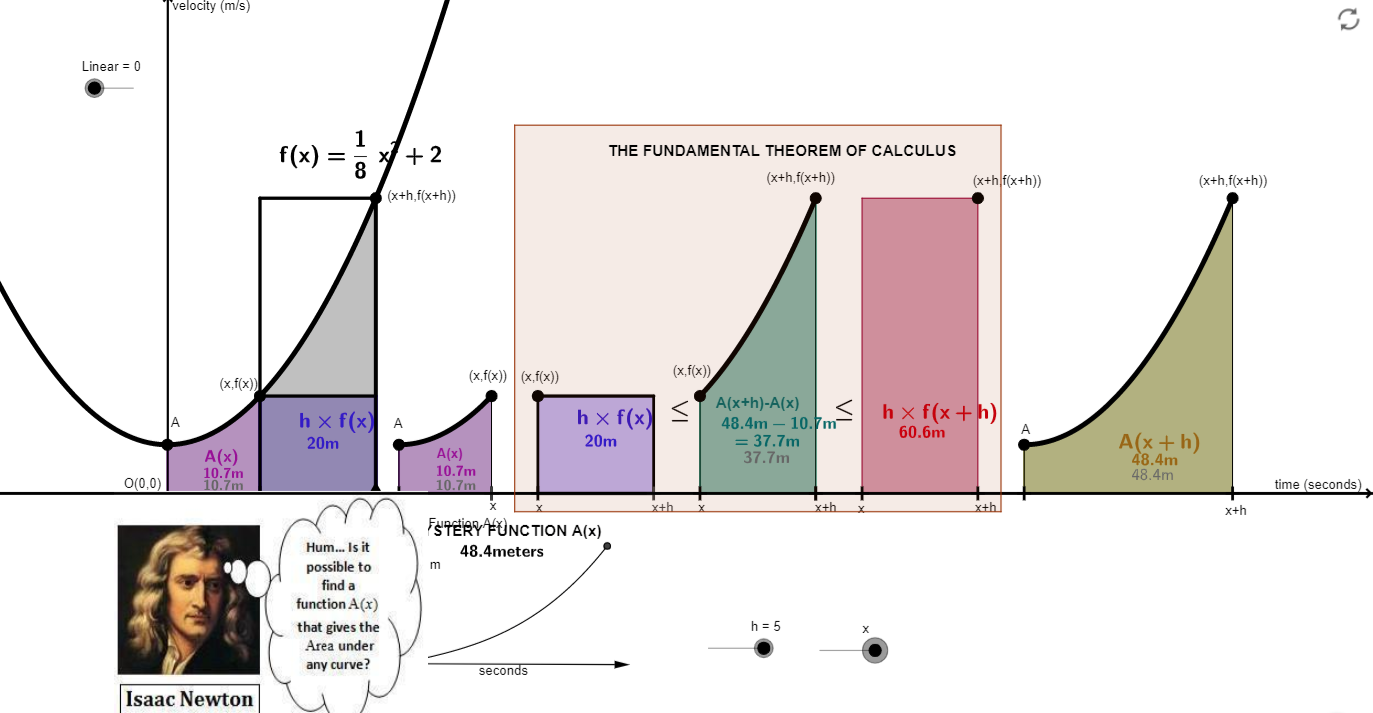
\includegraphics[width=0.8\linewidth]{img/image-20200427155419418.png}}
% \end{fullwidth}


\begin{example}

Evaluate the integral \[ \int_1^3 (x^2+3x)\,\mathrm{d}x\]

\end{example}
\vspace*{6\baselineskip}

\begin{example}

Evaluate the integral \[ \int_0^\pi \sin x \,\mathrm{d}x\]

\end{example}
\vspace*{6\baselineskip}

\begin{example}

Find the derivative of \[G(x)=\int_1^x (t^2-3t)\,dt\]

\end{example}
\vspace*{6\baselineskip}

\begin{example}

Find the derivative of \[G(x)=\int_1^{x^2} \cos(3t)\,dt\]

\end{example}
\vspace*{6\baselineskip}

\begin{example}

Find the derivative of \[G(x)=\int_x^1 \tan(t^2)\,dt\]

\end{example}
\vspace*{6\baselineskip}

\subsection{Practice}

\begin{exercise}

Evaluate the definite integral.

\begin{enumerate}
\item
  \(\displaystyle \int^2_{-1}(x^2-3x)\,dx\)
\item
  \(\displaystyle \int^3_{-2}(t+2)(t-3)dt\)
\end{enumerate}

\end{exercise}

\begin{exercise}

Find the derivative of the function.

\begin{enumerate}
\item
  \(\displaystyle f(x)=\frac{d}{dx}\int^x_3\sqrt{9-y^2}\,dy\)
\item
  \(\displaystyle f(x)=\frac{d}{dx}\int^{x^2}_0\sqrt{1-t^2}\,dt\)
\item
  \(\displaystyle f(x)=\frac{d}{dx}\int^1_{\cos x}\sqrt{1-t^2}\,dt\)
\end{enumerate}

\end{exercise}

